\section{Текст задания}
Сконфигурировать в своём домашнем каталоге репозитории svn и git и
загрузить в них начальную ревизию файлов с исходными кодами (в соответствии с выданным вариантом).

Воспроизвести последовательность команд для систем контроля версий svn и git,
осуществляющих операции над исходным кодом, приведённые на блок-схеме.

При составлении последовательности команд необходимо учитывать следующие условия:

\begin{itemize}
  \item Цвет элементов схемы указывает на пользователя, совершившего действие (красный - первый, синий - второй).
  \item Цифры над узлами - номер ревизии. Ревизии создаются последовательно.
  \item Необходимо разрешать конфликты между версиями, если они возникают.
\end{itemize}

\begin{figure}[H]
\centering
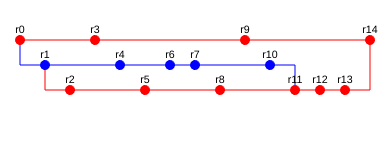
\includegraphics{./img/task.png}
\end{figure}

\section{Выполнение}
\subsection{Git}
\inputminted[breaklines]{bash}{../git.sh}
\subsection{Svn}
\inputminted[breaklines]{bash}{../svn.sh}

\section{Вывод}
В ходе выполнения данной лабораторной работы мы изучили
основы работы с системами контроля версий Git и Subversion.
Мы также поняли, что Git намного удобнее и понятнее, чем Subversion.
